\begin{document}

Conforme especificado até o momento, montou-se o experimento a fim de verificar o correto funcionamento da comunicação a partir do protocolo LIN. Os dados obtidos serão analisados gráfica e estatisticamente.

Uma captura do gráfico gerado a partir das leituras de tensão na linha está exposto na Figura \ref{fig:plot}, sendo que o início de uma mensagem é exibido. Várias informações podem ser obtidas apenas da análise dessa imagem.

\begin{figure}[H]
    \centering
    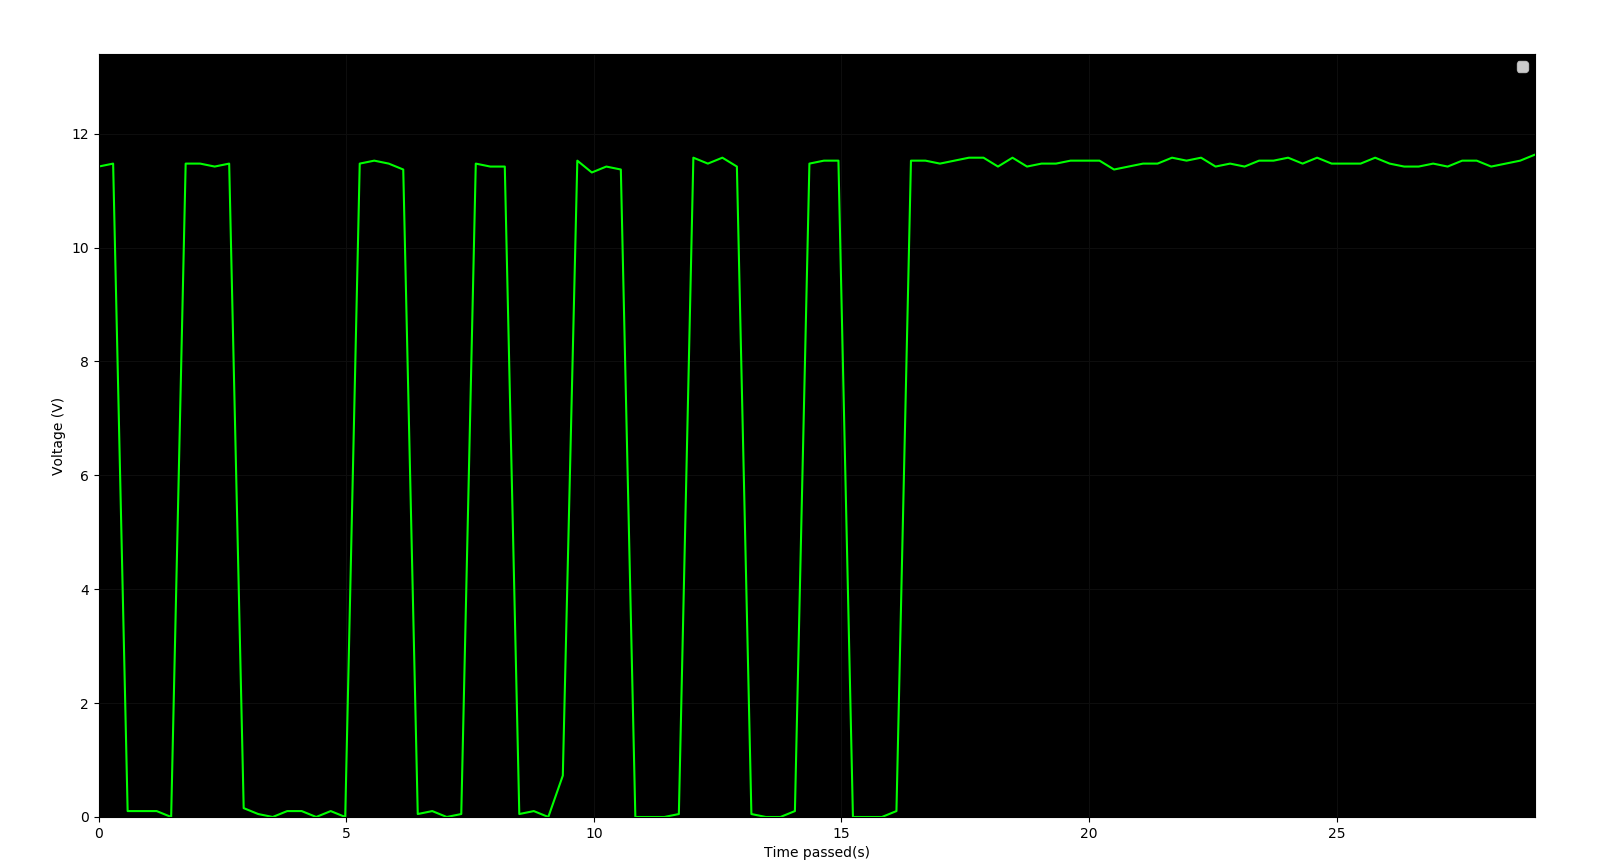
\includegraphics[width=.5\textwidth]{../figs/plot}
    \caption{Captura do gráfico gerado a partir dos dados obtidos.}
    \label{fig:plot}
\end{figure}

Primeiramente, percebe-se que os primeiros bits enviados são os de sincronização, representados pela alternância de zeros e uns lógicos (valor 0x55 em hexadecimal). Portanto, o MCP2003 \cite{datasheet:mcp2003} utiliza o sinal \textit{break} apenas para início de seu próprio sistema, como uma interrupção, não passando essa situação adiante. Uma vez que essa sinalização dura mais do que o tempo para envio e recebimento de um byte, é lógico pensar que essa informação não deve ser transmitida adiante, pois comprometeria a leitura pelo nó escravo.

Nota-se, também, que os níveis de tensão ficaram muito próximos de 12V e 0V, assim como prevê o protocolo. Ademais, enquanto nenhuma informação é enviada a tensão é mantida em nível alto, assim como acontece com a UART. 

Após essa análise qualitativa dos resultados obtidos, utilizou-se de uma análise estatística para averiguar a conformidade dos níveis de tensão da linha. Os valores estão expostos na Tabela \ref{tab:stats}. Esses números foram calculados a partir de mais de 500000 (quinhentas mil) leituras obtidas.

\begin{table}[htb]
\centering
\caption{Resultados estatísticos dos níveis de tensão.}
\label{tab:stats}
\begin{tabular}{clcc}
\textbf{Nível Lógico} & \textbf{Estatística} & \textbf{Quantizado} & \textbf{Tensão {[}V{]}} \\
\multirow{4}{*}{1}    & Média                & 227                 & 11,831                  \\
                      & Desvio-Padrão        & 2,414               & 0,127                   \\
                      & Mínimo               & 148                 & 7,714                   \\
                      & Máximo               & 236                 & 12,301                  \\
\multirow{4}{*}{0}    & Média                & 6                   & 0,313                   \\
                      & Desvio-Padrão        & 4,513               & 0,235                   \\
                      & Mínimo               & 0                   & 0                       \\
                      & Máximo               & 136                 & 7,088                  
\end{tabular}
\end{table}

Como é possível perceber, a tensão ficou em 11,831V na média para o nível lógico alto, com um desvio-padrão de 0,127V. Para o nível lógico baixo o valor ficou em 0,313V, com um desvio-padrão de 0,235V. Ambos os resultados demonstram que a tensão ficou bem estável ao longo desses níveis, além de estarem muito próximas aos valores nominais -- completamente aceitável dentro das faixas de operação.

O valor máximo para o nível zero e o valor mínimo para o nível alto, porém, ficam muito foras dos limites de operação e seriam interpretados como erros. O número 138 (quantizado) foi utilizado como separador por representar 40\% do máximo, que seria o limite para sair da faixa aceitável para o nível alto. Nesse caso, avaliou-se a incidência de valores fora das faixas aceitáveis de operação, como exibido na Tabela \ref{tab:out}. Os limites 92 e 138 representam as faixas aceitáveis de operação, por isso foram escolhidos. Os outros valores -- 20 e 210 -- foram utilizados para levar a uma situação mais extrema e verificar a quantidade de valores existentes próximos do limite.

\begin{table}[htb]
\centering
\caption{Ocorrência de valores fora da margem de aceitação.}
\label{tab:out}
\begin{tabular}{lcc}
\textbf{Faixa}                     & \textbf{Ocorrências} & \textbf{Percentual} \\
Valores entre 92 e 138 (inclusive) & 10                   & 0,0019\%            \\
Valores entre 20 e 210 (inclusive) & 36                   & 0,0068\%           
\end{tabular}
\end{table}

Percebe-se que a ocorrência de valores fora da faixa de operação é ínfima, com percentual de menos de 0,01\%. Possivelmente, esses dados são oriundos de medições feitas exatamente no momento em que a tensão estava passando de um nível alto para baixo ou vice-versa.

Desse modo, pôde-se avaliar o desempenho e particularidades do protocolo LIN, exibindo ótimos resultados apesar do baixo custo em comparação com outras alternativas para o mercado automobilístico.

\end{document}